\documentclass[12pt,a4paper]{article}
\usepackage[ascii]{inputenc}
\usepackage{amsmath}
\usepackage{amsfonts}
\usepackage{amssymb}
\usepackage{graphicx}
\usepackage[dutch]{babel}
\usepackage{hyperref}
\usepackage{geometry}
\usepackage{tabularx}
\usepackage{parskip}


\geometry{margin=1in}
\author{Nikki van der Gouw s4463412}
\title{Handleiding Wheelie}
\begin{document}
\maketitle
\newpage
\tableofcontents
\newpage

\section{Introductie}
In deze handleiding vind je alles wat nodig is om ook zelf de zelfbalancerende robot "Wheelie" te kunnen maken. De handleiding is in 3 onderdelen te verdelen: de montage van de robot, het installeren van de software en het gebruik van Wheelie. 

\section{Hardware}
Voor dit project is gebruik gemaakt van de volgende onderdelen:
\begin{table}[!h]
	\begin{tabularx}{\textwidth}{|X|X|}	
		\hline \multicolumn{2}{|c|}{\textbf{adafruit BNO055 (Absolute Orienation Sensor)}}	\\	
		\hline \textbf{Aansluiting op onderdeel} & \textbf{Aansluiting op Arduino} \\ 
		\hline VIN & 3.5V \\ 
		\hline GND & GND\\ 
		\hline SCL & A5 \\  
		\hline SDA & A4 \\
		\hline \multicolumn{2}{|c|}{\textbf{nRF8001 (Bluetooth LE)}}	\\	 
		\hline \textbf{Aansluiting op onderdeel} & \textbf{Aansluiting op Arduino} \\
		\hline VIN & 5v \\
		\hline GND & GND \\
		\hline SCK & 13 \\
		\hline MISO & 12 \\
		\hline MOSI & 11 \\
		\hline REQ & 10 \\
		\hline RST & 9 \\
		\hline RDY & 2 \\
		\hline \multicolumn{2}{|c|}{\textbf{L298N (Dual H-bridge Motor Controller)}}	\\	 
		\hline \textbf{Aansluiting op onderdeel} & \textbf{Aansluiting op Arduino} \\
		\hline GND & GND \\
		\hline ENA & 5  \\
		\hline ENB & 6 \\
		\hline IN1 & 3 \\
		\hline IN2 & 4 \\
		\hline IN3 & 7 \\
		\hline IN4 & 8 \\
		\hline \textbf{Aansluiting op onderdeel} & \textbf{Aansluiting op motor L} \\
		\hline OUT1 & witte draad \\
		\hline OUT2 & blauwe draad \\
		\hline \textbf{Aansluiting op onderdeel} & \textbf{Aansluiting op motor R} \\
		\hline OUT3 & blauwe draad \\
		\hline OUT4 & zwarte draad \\
		\hline \multicolumn{2}{|c|}{\textbf{Batterijhouder}}\\	 
		\hline \textbf{Aansluiting op onderdeel} & \textbf{Aansluiting op Arduino} \\
		\hline grote ronde stekker & DC input \\
		\hline \textbf{Aansluiting op onderdeel} & \textbf{Aansluiting op motor controller} \\
		\hline zwarte draad & GND \\
		\hline rode draad & 12V \\		
		\hline		
	\end{tabularx} 
	\caption{Arduino aansluitingen}
	\label{tbl:Aansluitingen}
\end{table}

\begin{tabular}{|c|c|}
	\hline Onderdelen & Aantal \\ 
	\hline Arduino UNO & 1 \\ 
	\hline  &  \\ 
	\hline  &  \\ 
	\hline  &  \\ 
	\hline 
\end{tabular} 

Aansluitingen

\section{Software}
\subsection{Arduino}
Voor dit project is gebruik gemaakt van de Arduino IDE ARDUINO (ARDUINO 1.6.7). De laatste versie van ARDUINO is te downloaden op onderstaande link: \url{https://www.arduino.cc/en/Main/Software}. Deze software is beschrikbaar voor Windows Mac OS X en Linux. Op de website van Arduino staan ook instructies voor het installeren van de IDE en verdere documentatie \cite{ARDUINO_getting started}.

Hieronder vind je een tabel met alle gebruikte libraries voor dit project.
Eerst komen alle libraries die gebruikt zijn in de code voor de arduino.

\begin{table}[h]
	\begin{tabularx}{\textwidth}{|l|l|X|}
	\hline \textbf{Bibliotheek} & \textbf{Versie} & \textbf{Download link}  \\ 
	\hline Wire & 1.0 & - \\ 
	\hline SPI & 1.0 & - \\ 
	\hline SoftwareSerial & 1.0 & - \\ 
	\hline Adafruit\_Sensor & 1.0.2 &  \url{https://github.com/adafruit/Adafruit_Sensor/archive/master.zip}  \\ 
	\hline Adafruit\_BNO055 & 1.1.2 & \url{https://github.com/adafruit/Adafruit_BNO055/archive/master.zip} \\ 
	\hline Adafruit\_BLE\_UART & 1.0.0 & \url{https://github.com/adafruit/Adafruit_nRF8001/archive/master.zip }\\ 
	\hline		
	\end{tabularx} 
	\caption{Arduino libraries}
	\label{tbl:Download_link}
\end{table}

De libraries Wire, SPI, en SoftwareSerial worden standaard bijgeleverd bij de Arduino IDE. De overige libraries moeten handmatig toegevoegd worden. De download links in Tabel \ref{tbl:Download_link} verwijzen naar een .zip bestand met de gewenste library. De libraries kun je aan de Arduino IDE toevoegen door in het menu van de IDE te klikken op $$ \text{Sketch} \rightarrow \text{Include Library }\rightarrow \text{Add .ZIP Library ..}$$ en hier de gewenste .zip bestand te selecteren.
\begin{figure}[h]
\centering
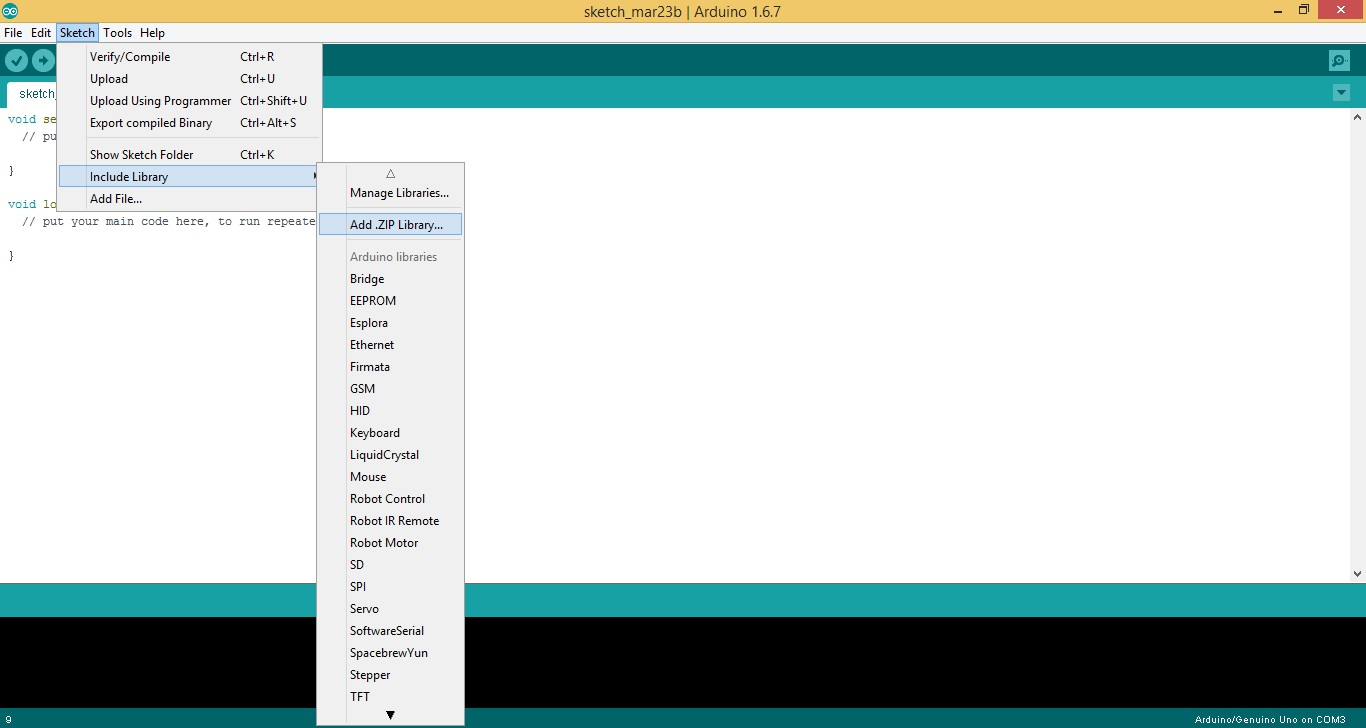
\includegraphics[width=0.7\linewidth]{Add_ZIP}
\caption{voeg een library toe aan de Arduino IDE}
\label{fig:Add_ZIP}
\end{figure}

Unzip de source code. 
open de code
Check de aansuitingen van de arduino.

\newpage
\begin{thebibliography}{9}
\bibitem{BLE_tutorial}
Townsend, K. (2015, 04 mei). Getting Started with the nRF8001 Bluefruit LE Breakout. 
Geraadpleegd van \url{https://learn.adafruit.com/getting-started-with-the-nrf8001-bluefruit-le-breakout/}

\bibitem{BLE_voorbeeldapp}
tdicola (2015, 06 oktober). BTLETest. Geraadpleegd van \url{https://github.com/tdicola/BTLETest/}

\bibitem{acc_tutorial}
zagGrad (2011, 10 januari). ADXL345 Quickstart Guide. Geraadpleegd van \url{https://www.sparkfun.com/tutorials/240}

\bibitem{BLE_specs}
KIWI electronics. (z.j.). 
BLUEFRUIT LE - BLUETOOTH LOW ENERGY (BLE 4.0) - NRF8001 BREAKOUT. Geraadpleegd van \url{https://www.kiwi-electronics.nl/bluefruit-le-bluetooth-low-energy-ble-4-0-nRF8001-breakout}

\bibitem{UNO_specs}
ARDUINO. (z.j). Arduino UNO \& Genuino UNO. Geraadpleegd van \url{https://www.arduino.cc/en/Main/ArduinoBoardUno}

\bibitem{acc_specs}
SparkFun. (z.j). SparkFun Triple Axis Accelerometer Breakout - ADXL345. Geraadpleegd van \url{https://www.sparkfun.com/products/9836}

\bibitem{DIY_specs}
DX. (z.j). DIY Intelligent Tortoise Smart Wheel Robot Module-Black. Geraadpleegd van 
\url{http://www.dx.com/p/diy-intelligent-tortoise-smart-wheel-robot-module-173668?tc=EUR&gclid=CI7qtbm5p78CFa_KtAodTSgAVA#.VvvjLeKLTIW}

\bibitem{camera_specs}
AI-Ball. (z.j). What is an AI-ball? Geraadpleegd van
\url{http://www.thumbdrive.com/aiball/intro.html}

\bibitem{Balancing_robot}
Dorweiler, J. (2012, 27 mei). Balancing Robot. Geraadpleeg van
\url{http://www.transistor.io/balancing-robot.html}

\bibitem{voorbeeld2}
Short, J. (z.j). How to Build a Self-Balancing Autonomous Arduino Bot. Geraadpleegd van 
\url{http://makezine.com/projects/arduroller-self-balancing-robot/}

\bibitem{ARDUINO_getting started}
ARDUINO. (z.j). Getting Started with Arduino. Geraadpleegd van \url{https://www.arduino.cc/en/Guide/HomePage}
\end{thebibliography}

\end{document}